%% VIth_SPHERIC_paper_tempalte.tex
%% V1.0
%% 2003/03/20
%% by Benedict Rogers
%% courtesy of nicolas.grenier@ec-nantes
%% courtesy of pierre.maruzewski@epfl.ch
%%
%% NOTE: This text file uses MS Windows line feed conventions. When (human)
%% reading this file on other platforms, you may have to use a text
%% editor that can handle lines terminated by the MS Windows line feed
%% characters (0x0D 0x0A).

% Note that the a4paper option is mainly intended so that authors in
% countries using A4 can easily print to A4 and see how their papers will
% look in print. Authors are encouraged to use U.S.
%
% Also note that the "draftcls" or "draftclsnofoot", not "draft", option
% should be used if it is desired that the figures are to be displayed in
% draft mode.
%
% This paper can be formatted using the peerreviewca
% (instead of conference) mode.
\documentclass[a4paper,conference]{IEEEtran}
% If the IEEEtran.cls has not been installed into the LaTeX system files,
% manually specify the path to it:
% \documentclass[conference]{../sty/IEEEtran}

% Dimensions of margins (DO NOT MODIFY THEM)
\setlength{\textheight}    {23.4cm}%
\setlength{\topmargin}     {-0.8cm}%
\setlength{\headheight}    {0.6cm}%
\setlength{\headsep}       {0.9cm}%

% some very useful LaTeX packages include:

\usepackage{cite}      % Written by Donald Arseneau
                        % V1.6 and later of IEEEtran pre-defines the format
                        % of the cite.sty package \cite{} output to follow
                        % that of IEEE. Loading the cite package will
                        % result in citation numbers being automatically
                        % sorted and properly "ranged". i.e.,
                        % [1], [9], [2], [7], [5], [6]
                        % (without using cite.sty)
                        % will become:
                        % [1], [2], [5]--[7], [9] (using cite.sty)
                        % cite.sty's \cite will automatically add leading
                        % space, if needed. Use cite.sty's noadjust option
                        % (cite.sty V3.8 and later) if you want to turn this
                        % off. cite.sty is already installed on most LaTeX
                        % systems. The latest version can be obtained at:
                        % http://www.ctan.org/tex-archive/macros/latex/contrib/supported/cite/

\usepackage{graphicx}  % Written by David Carlisle and Sebastian Rahtz
                        % Required if you want graphics, photos, etc.
                        % graphicx.sty is already installed on most LaTeX
                        % systems. The latest version and documentation can
                        % be obtained at:
                        % http://www.ctan.org/tex-archive/macros/latex/required/graphics/
                        % Another good source of documentation is "Using
                        % Imported Graphics in LaTeX2e" by Keith Reckdahl
                        % which can be found as esplatex.ps and epslatex.pdf
                        % at: http://www.ctan.org/tex-archive/info/
% NOTE: for dual use with latex and pdflatex, instead load graphicx like:
%\ifx\pdfoutput\undefined
%\usepackage{graphicx}
%\else
%\usepackage[pdftex]{graphicx}
%\fi

% However, be warned that pdflatex will require graphics to be in PDF
% (not EPS) format and will preclude the use of PostScript based LaTeX
% packages such as psfrag.sty and pstricks.sty. IEEE conferences typically
% allow PDF graphics (and hence pdfLaTeX). However, IEEE journals do not
% (yet) allow image formats other than EPS or TIFF. Therefore, authors of
% journal papers should use traditional LaTeX with EPS graphics.
%
% The path(s) to the graphics files can also be declared: e.g.,
% \graphicspath{{../eps/}{../ps/}}
% if the graphics files are not located in the same directory as the
% .tex file. This can be done in each branch of the conditional above
% (after graphicx is loaded) to handle the EPS and PDF cases separately.
% In this way, full path information will not have to be specified in
% each \includegraphics command.
%
% Note that, when switching from latex to pdflatex and vice-versa, the new
% compiler will have to be run twice to clear some warnings.

\usepackage{wasysym}
%\usepackage{psfrag}    % Written by Craig Barratt, Michael C. Grant,
                        % and David Carlisle
                        % This package allows you to substitute LaTeX
                        % commands for text in imported EPS graphic files.
                        % In this way, LaTeX symbols can be placed into
                        % graphics that have been generated by other
                        % applications. You must use latex->dvips->ps2pdf
                        % workflow (not direct pdf output from pdflatex) if
                        % you wish to use this capability because it works
                        % via some PostScript tricks. Alternatively, the
                        % graphics could be processed as separate files via
                        % psfrag and dvips, then converted to PDF for
                        % inclusion in the main file which uses pdflatex.
                        % Docs are in "The PSfrag System" by Michael C. Grant
                        % and David Carlisle. There is also some information
                        % about using psfrag in "Using Imported Graphics in
                        % LaTeX2e" by Keith Reckdahl which documents the
                        % graphicx package (see above). The psfrag package
                        % and documentation can be obtained at:
                        % http://www.ctan.org/tex-archive/macros/latex/contrib/supported/psfrag/

%\usepackage{subfigure} % Written by Steven Douglas Cochran
                        % This package makes it easy to put subfigures
                        % in your figures. i.e., "figure 1a and 1b"
                        % Docs are in "Using Imported Graphics in LaTeX2e"
                        % by Keith Reckdahl which also documents the graphicx
                        % package (see above). subfigure.sty is already
                        % installed on most LaTeX systems. The latest version
                        % and documentation can be obtained at:
                        % http://www.ctan.org/tex-archive/macros/latex/contrib/supported/subfigure/

%\usepackage{url}       % Written by Donald Arseneau
                        % Provides better support for handling and breaking
                        % URLs. url.sty is already installed on most LaTeX
                        % systems. The latest version can be obtained at:
                        % http://www.ctan.org/tex-archive/macros/latex/contrib/other/misc/
                        % Read the url.sty source comments for usage information.

%\usepackage{stfloats}  % Written by Sigitas Tolusis
                        % Gives LaTeX2e the ability to do double column
                        % floats at the bottom of the page as well as the top.
                        % (e.g., "\begin{figure*}[!b]" is not normally
                        % possible in LaTeX2e). This is an invasive package
                        % which rewrites many portions of the LaTeX2e output
                        % routines. It may not work with other packages that
                        % modify the LaTeX2e output routine and/or with other
                        % versions of LaTeX. The latest version and
                        % documentation can be obtained at:
                        % http://www.ctan.org/tex-archive/macros/latex/contrib/supported/sttools/
                        % Documentation is contained in the stfloats.sty
                        % comments as well as in the presfull.pdf file.
                        % Do not use the stfloats baselinefloat ability as
                        % IEEE does not allow \baselineskip to stretch.
                        % Authors submitting work to the IEEE should note
                        % that IEEE rarely uses double column equations and
                        % that authors should try to avoid such use.
                        % Do not be tempted to use the cuted.sty or
                        % midfloat.sty package (by the same author) as IEEE
                        % does not format its papers in such ways.

% \usepackage{amsmath}   % From the American Mathematical Society
                        % A popular package that provides many helpful commands
                        % for dealing with mathematics. Note that the AMSmath
                        % package sets \interdisplaylinepenalty to 10000 thus
                        % preventing page breaks from occurring within multiline
                        % equations. Use:
%\interdisplaylinepenalty=2500
                        % after loading amsmath to restore such page breaks
                        % as IEEEtran.cls normally does. amsmath.sty is already
                        % installed on most LaTeX systems. The latest version
                        % and documentation can be obtained at:
                        % http://www.ctan.org/tex-archive/macros/latex/required/amslatex/math/



% Other popular packages for formatting tables and equations include:

%\usepackage{array}
% Frank Mittelbach's and David Carlisle's array.sty which improves the
% LaTeX2e array and tabular environments to provide better appearances and
% additional user controls. array.sty is already installed on most systems.
% The latest version and documentation can be obtained at:
% http://www.ctan.org/tex-archive/macros/latex/required/tools/

% Mark Wooding's extremely powerful MDW tools, especially mdwmath.sty and
% mdwtab.sty which are used to format equations and tables, respectively.
% The MDWtools set is already installed on most LaTeX systems. The lastest
% version and documentation is available at:
% http://www.ctan.org/tex-archive/macros/latex/contrib/supported/mdwtools/


% V1.6 of IEEEtran contains the IEEEeqnarray family of commands that can
% be used to generate multiline equations as well as matrices, tables, etc.


% Also of notable interest:

% Scott Pakin's eqparbox package for creating (automatically sized) equal
% width boxes. Available:
% http://www.ctan.org/tex-archive/macros/latex/contrib/supported/eqparbox/



% Notes on hyperref:
% IEEEtran.cls attempts to be compliant with the hyperref package, written
% by Heiko Oberdiek and Sebastian Rahtz, which provides hyperlinks within
% a document as well as an index for PDF files (produced via pdflatex).
% However, it is a tad difficult to properly interface LaTeX classes and
% packages with this (necessarily) complex and invasive package. It is
% recommended that hyperref not be used for work that is to be submitted
% to the IEEE. Users who wish to use hyperref *must* ensure that their
% hyperref version is 6.72u or later *and* IEEEtran.cls is version 1.6b
% or later. The latest version of hyperref can be obtained at:
%
% http://www.ctan.org/tex-archive/macros/latex/contrib/supported/hyperref/
%
% Also, be aware that cite.sty (as of version 3.9, 11/2001) and hyperref.sty
% (as of version 6.72t, 2002/07/25) do not work optimally together.
% To mediate the differences between these two packages, IEEEtran.cls, as
% of v1.6b, predefines a command that fools hyperref into thinking that
% the natbib package is being used - causing it not to modify the existing
% citation commands, and allowing cite.sty to operate as normal. However,
% as a result, citation numbers will not be hyperlinked. Another side effect
% of this approach is that the natbib.sty package will not properly load
% under IEEEtran.cls. However, current versions of natbib are not capable
% of compressing and sorting citation numbers in IEEE's style - so this
% should not be an issue. If, for some strange reason, the user wants to
% load natbib.sty under IEEEtran.cls, the following code must be placed
% before natbib.sty can be loaded:
%
% \makeatletter
% \let\NAT@parse\undefined
% \makeatother
%
% Hyperref should be loaded differently depending on whether pdflatex
% or traditional latex is being used:
%
%\ifx\pdfoutput\undefined
%\usepackage[hypertex]{hyperref}
%\else
%\usepackage[pdftex,hypertexnames=false]{hyperref}
%\fi
%
% Pdflatex produces superior hyperref results and is the recommended
% compiler for such use.



% *** Do not adjust lengths that control margins, column widths, etc. ***
% *** Do not use packages that alter fonts (such as pslatex).         ***
% There should be no need to do such things with IEEEtran.cls V1.6 and later.


% correct bad hyphenation here
\hyphenation{op-tical net-works semi-conduc-tor IEEEtran}



\usepackage{fancyheadings}
\usepackage{float}
\usepackage{afterpage}
\usepackage{subfig}
\pagestyle{fancy}

\lhead{$10^{th}$ international SPHERIC workshop}
\rhead{Parma, Italy, June, 2015}
\cfoot{} % to avoid page numbering

\newcommand{\OF}{OpenFOAM\textsuperscript{\textregistered}}
\newcommand{\FF}{Fluent\textsuperscript{\textregistered}}
\newcommand{\tauB}{\underline{\underline{\boldsymbol{\tau}}}}
\newcommand{\vv}{\mathbf{v}}
\newcommand{\xx}{\mathbf{x}}
\newcommand{\aaa}{\mathbf{a}}
\newcommand{\ww}{\mathbf{w}}
\newcommand{\gb}{\mathbf{g}}
\newcommand{\nn}{\mathbf{n}}
\newcommand{\yy}{\mathbf{y}}
\newcommand{\Mat}{Matlab{\small$^{\textregistered}$}}


\begin{document}

% paper title
\title{Free surface application of the PFEM (particles + finite elements) methodology to submerged cylinders}


% author names and affiliations
% use a multiple column layout for up to three different
% affiliations
\author{\IEEEauthorblockN{Leo M. Gonz\'{a}lez\\
                        Esteban Ferrer}
\IEEEauthorblockA{Universidad Polit\'{e}cnica de Madrid (UPM)\\
Madrid, Spain\\
leo.gonzalez@upm.es\\
esteban.ferrer@upm.es}
\and
\IEEEauthorblockN{Juan M. Gimenez}
\IEEEauthorblockA{CIMEC - CONICET\\
Universidad Nacional del Litoral (UNL)\\
Santa Fe, Argentina\\
jmarcelogimenez@gmail.com}
}

% use only for invited papers
%\specialpapernotice{(Invited Paper)}

% make the title area
\maketitle

\begin{abstract}
In this paper, a new generation of the particle method known as Particle Finite Element Method (PFEM-2) \cite{Idelsohn04}, which combines convective particle movement and a fixed mesh resolution, is applied to a 2D flow past a circular cylinder intersecting or close to a free surface at Reynolds 180 \cite{Bouscasse14}. To accomplish this task, different improved versions of discontinuous and continuous enriched basis functions for the pressure field have been developed \cite{Gimenez2015186} to capture the free surface dynamics without artificial diffusion or undesired numerical effects. The well-known numerical properties of PFEM-2 such as using larger time steps when compared to other similar numerical tools which implies shorter computational times while maintaining the accuracy of the computation will be checked in this case. In particular, for this free surface cylinder, the wake behavior for Froude numbers between 0.3 and 2.0 are examined.
The PFEM-2 technique allows for a very little diffusive computation of the free surface evolution, even while breaking and fragmentation may occur. Vorticity shed by the cylinder, vortex generation due to free surface breaking, mixing processes, and drag and lift coefficients behavior are quantified. It has been found that, for small gap ratios, the classical von Karman vortex shedding from the cylinder does not take place for most of the Froude numbers considered. In turn, moderate vortex shedding occurs, departing not from the cylinder but originating from wave breaking at the free surface. This shedding takes places simultaneously with the transport of free surface fluid elements into the bulk of the fluid. In some combinations of Froude number and submergence ratio, a vorticity layer remains spatially localized between the cylinder and the free surface and a large recirculating wake area develops, which eventually gets detached after several shedding cycles, being advected downstream. In order to study the stability of these kind of complex flows and the tendency to develop absolute and convective instabilities, a Dynamic Mode Decomposition (DMD) stability analysis has been used. To the authors knowledge this has been the first time that a flow in the presence of free surface has been analyzed by this of technique. The DMD stability analysis captures perfectly either the growth or the damping tendency of the flow as well as the most relevant frequencies. This study is performed using a number of snapshots computed by the described PFEM methodology which are subsequently analyzed by a Dynamic Mode Decomposition (DMD) stability analysis.
\end{abstract}


\section{Introduction}

The goal of this work is to extend the possibilities of PFEM-2 to complex problems where free surface is present. In order to do that, the flow around a circular cylinder in the presence of free surface has been investigated at low Reynolds numbers with this numerical method. In our case, the Reynolds number is limited to 180, and consequently the spectrum of industrial applications is not obvious. However, problems like the containment of oil spills by mechanical barriers \cite{Amini20081479} or the variety of power generator designs that operate close to the free surface and are driven by VIV (Vortex Induced Vibrations), constitute a framework where the concepts that are numerically simulated in this work could be potentially applied. Assuming a vast literature concerning the study of 2D laminar flows around circular cylinders without free surface, the presence of this free surface boundary limits the number of previous publications. An interesting comparison was performed by Reichl et al. \cite{Reichl05} between the flow around submerged cylinders at $Re=180$ computed by FLUENT and the experimental results obtained by Sheridan and Rockwell \cite{sheridan_etal_pof1995_metastable_cylinder_fs,SHERIDAN_ROCKWELL_JFM1997} at large Reynolds numbers. The difference in the Reynolds numbers could be justified by the fact that is the Froude number the non-dimensional number that really affects these kind of flows. An important contribution to these kind of problems is the possibility of performing a stability analysis of the flow and the comparison with the classical case where no free surface is affecting. A typical case where the cylinder is partially submerged is studied by Triantafyllou and Dimas \cite{Dimas89}, where the concluded that the presence of the free surface has a stabilizing effect in the global flow. The PFEM-2 treatment of the free surface described by Gimenez in \cite{Gimenez2015186}, permits an adequate study of the free surface evolution, even in these cases where proximity of the cylinder to the free surface may induce fragmentation. Another important numerical study was performed by Bouscasse \cite{Bouscasse14}, where a suitable method for highly nonlinear free surface flows such as the SPH numerical method \cite{Mon77} is used to compute a vast combination of Reynolds and Froude numbers.
The stability of these flows was studied by Dimas in \cite{Dimas89}, using the Rayleigh equation to quantify the transition from a convective to global stability when an analytic and steady parallel velocity profile was used as baseflow and viscous effects were neglected. This stability analysis study is performed using the Froude number as the principal parameter and the transition from convective to absolute is found at $Fr=2.5$. More complex linear stability analysis of complex flows have been performed during the last decades taking all components of the velocity into account and keeping the viscous terms in the global formulation. The classical methodology, known as biglobal stability analysis, was to linearize the Navier-Stokes equations using stationary or periodic flows as baseflows, and perturbing the solution in order to transform the problem into a generalized eigenvalue problem. Alternatively the modern Dynamic Mode Decomposition Technique, based on the construction of a Krylov subspace using snapshots issued from numerical simulations, permits an adequate methodology to analyze non-stationary flows as the ones studied here. In recent years, the snapshot based technique Dynamic Mode Decomposition (DMD), has seen an increased popularity \cite{DMDSchmid,princeton} and has been applied to a variety of flows including numerical and experimental data, e.g. \cite{Bagheri_Cyl,Mezic_koopman,Rowley_JFM,Soria_DMD}. The formulation retained here can be found in \cite{DMDSchmid}, but other algorithms have also been proposed \cite{princeton,SparsityDMD}. In addition, we note that the temporal framework for the study of flow instability is retained, but that the DMD with spatial snapshots is also possible \cite{DMDSchmid}. It was shown by Mezic \cite{Mezic_koopman}, Rowley \textit{et al.} \cite{Rowley_JFM} and more recently by Bagheri \cite{Bagheri_Cyl} that the modes resulting from the DMD algorithm are approximations of Koopman modes. Koopman operators are infinite dimensional linear operators capable of describing nonlinear processes. Some of the associated infinite number of modes related to this operator may be approximated through the DMD decomposition \cite{Mezic_koopman}.

\section{PFEM formulation}\label{GeneralFor}

In this section a brief review of the PFEM-2 methodology used to numerically simulate the dynamics of two incompressible immiscible fluids. The governing equations are the incompressible Navier-Stokes equations for both fluids, which are supplemented with the conventional boundary conditions on solid and/or open boundaries. The computational domain $\Omega$ contains both fluids, the first one, denoted by subscript 1, and the second one with its corresponding variables denoted by the subscript 2 with densities and viscosities $\rho_i$ and $\mu_i$ $(i=1,2)$, respectively. The governing equations, written in a Lagrangian framework, are:

\begin{eqnarray}
% \nonumber to remove numbering (before each equation)
  \nabla \cdot \mathbf{v} &=& 0 \label{eq:continuity} \\
  \nonumber \\
  \rho\frac{D\mathbf{v}}{Dt} &=& -\nabla p + \mu \nabla^2 \mathbf{v} + \mathbf{f}\label{eq:momentum}
\end{eqnarray}

As expected, a kinematic problem based on the particle formulation has to be solved at each time step. Here $\mathbf{v}$, $p$ are the velocity and fluid pressure and $\mathbf{f}$ is an external body force (normally gravity $\rho \mathbf{g}$ and/or inertial force).

In order to decouple the unknown fields: velocity and pressure, segregated or projection methods like fractional step were implemented in PFEM-2. In our case two different fluids (air and water) separated by an interface are considered, each particle $p$ carries the information of the fluid to which it was initially assigned. This quantity, represented by a scalar function $\lambda_p$, assumes integer values $1$ or $-1$ depending if it belongs to the first or second fluid. This value is advected, adding one equation to the kinematic integration stage:

\begin{equation}\label{Free_surface}
    \frac{D\lambda}{Dt}=0,
\end{equation}

i.e. each particle keeps its marker value during the entire simulation. This function is projected to the mesh nodes to determine the free-surface position. Mesh nodes thus obtain real values after the projection which are different to the integer values $\pm1$ that the particles transport. The free-surface interface is defined as the set of points that satisfy the equation $\lambda=0$, and a Heaviside function is used to determinate intensive properties (density and viscosity) on the nodes.

\begin{figure}[ht]
  \centering
  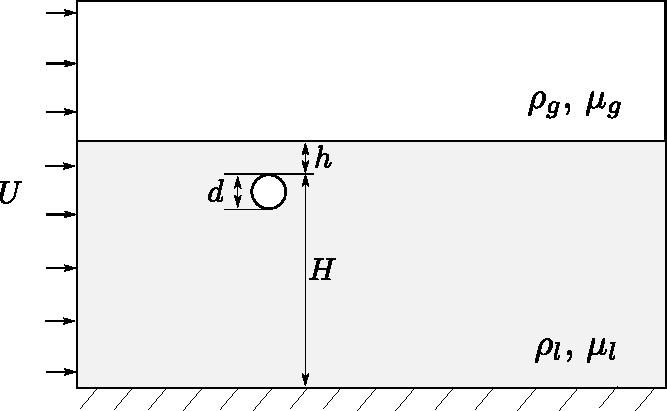
\includegraphics[width=0.9\columnwidth]{images_10thspheric/config.pdf}
  \caption{Case configuration, initial and boundary conditions.}
  \label{fg:config}
\end{figure}


%Following a fractional step, the momentum equation is discretized in time in such a way that it firstly predicts a velocity using the old value of the pressure (the pressure at the old time step) and, after correcting this predicted velocity with the updated pressure that arises from applying the divergence operator to the correction equation, getting a Poisson like equation for the pressure.
%Similarly to other Navier-Stokes algorithms, there are three main steps: predictor, Poisson equation and correction. Predictor step is done by four sub-steps:
%
%\begin{enumerate}
%  \item An acceleration calculation stage over the mesh.
%  \item The X-IVAS stage to convect the fluid properties using the particles.
%  \item The projection of the particle data to the mesh nodes.
%  \item The implicit calculation of the diffusion term.
%\end{enumerate}

%The predictor step ends with a predicted velocity $\widehat\vv^{n+1}$ on the mesh. After that, a Poisson equation to find the current pressure $p^{n+1}$ is solved. Finally, the velocity prediction is corrected to find the zero divergence field $\vv^{n+1}$.

In \cite{gimenezgonzalez2014,Gimenez2015186}, a complete description of the general algorithm that PFEM-2 follows in order to compute a complete time step and the methodology followed to capture the free surface can be found.

\section{Dynamic Mode Decomposition Analysis}



%Namely, DMD modes approximate Koopman modes \cite{Mezic_koopman}, which are structures resulting from the spectral analysis of a Koopman operator. The latter is defined as an infinite dimensional linear operator capable of approximating a nonlinear operator \cite{Rowley_JFM}, further details are provided in
%section \ref{sec:dmd_theory}.

Schmid \cite{DMDSchmid} described in detail the DMD technique and hence only a summary of the algorithm is described here. Given a sequence of 1 to $N$ flowfield snapshots (e.g. taking one or all variables of the flow field), one can construct the following matrix:
\begin{equation}\label{eq:dmd_1}
 {\mathbf{V}_1}^N=\{\mathbf{v(t_1)},\mathbf{v(t_2)},..,\mathbf{v(t_N)}\},
 \end{equation}
 where subindex and superindex denote the first and last values of the sequence, respectively.
  Let us note that this data needs to be ordered, and that the snapshots require a constant sampling time $\Delta\tau$ such that: $t_{j+1}=t_j+\Delta\tau$ for all $j=1,..,N$. In the case of linear stability analysis and within the exponential growth region, one can define a linear operator $\mathbf{A}$ (i.e. a numerical approximation of the linearised NS operator)  between snapshots such that $v(t_{j+1})=\mathbf{A}v(t_j)$, one can rewrite Eq. \ref{eq:dmd_1} as a Krylov sequence \cite{Saad:92}:
 \begin{equation}\label{eq:dmd_2}
 {\mathbf{V}_1}^N=\{\mathbf{v(t_1)},\mathbf{A}\mathbf{v(t_1)},..,\mathbf{A}^{N-1}\mathbf{v(t_1)}\}.%=\{\mathbf{v(t_1)},\mathbf{A}\mathbf{v(t_1)},..,\mathbf{A}\mathbf{v(t_{N-1})}\}.
 \end{equation}
   It is easy to see that for an ordered sequence, Eq. \ref{eq:dmd_2} can be equated to Eq. \ref{eq:dmd_1}, to lead:
  \begin{equation}\label{eq:dmd_2bis}
  \mathbf{A}\{\mathbf{v(t_1)},\mathbf{v(t_2)},..,\mathbf{v(t_{N-1})}\}=\{\mathbf{v(t_2)},\mathbf{v(t_3)},..,\mathbf{v(t_N)}\},
 \end{equation}
 which can be written in matrix form as:
  \begin{equation}\label{eq:dmd_3}
   \mathbf{A}{\mathbf{V}_1}^{N-1}={\mathbf{V}_2}^{N}.
  \end{equation}
%
%The matrix $\mathbf{A}$ represents the matrix exponential of the nonlinear operator describing the Navier-Stokes equations; i.e. $\mathbf{{v}}(t_{j+1})=e^{\mathbf{B}\Delta t}\mathbf{{v}}(t_j)$, where $\mathbf{A}= e^{\mathbf{B}\Delta t}$ and $\mathbf{B}$ represents the numerically discretised nonlinear Navier-Stokes operator.
%\textcolor[rgb]{1.00,0.00,0.00}{This approximation is only exact for linear systems (i.e. as the ones considered in this paper for the exponential growth regime). However,}
%for non-linear systems (i.e. Navier-Stokes equations in the saturated regime) described by $\mathbf{A}$,

The algorithm continues by obtaining the Singular Value Decomposition (SVD) of the matrix ${\mathbf{V}_1}^{N-1}=\mathbf{U}\mathbf{\Sigma}\mathbf{W}^H$, where the superscript $H$ denotes the conjugate transpose. Replacing the SVD definition into Eq. \ref{eq:dmd_3}, leads to $\mathbf{A}\mathbf{U}\Sigma\mathbf{W}^H={\mathbf{V}_2}^{N}$. To find the reduced matrix $\mathbf{\widetilde{S}}$ associated to the initial system described by $\mathbf{A}$, it suffices to rewrite the previous equality as:
  \begin{equation}\label{eq:dmd_4}
   \mathbf{\widetilde{S}}=\mathbf{U}^H\mathbf{A}{\mathbf{U}}=\mathbf{U}^H{\mathbf{V}_2}^{N}\mathbf{W}\mathbf{\Sigma}^{-1}.
  \end{equation}
  Inspection of Eq. \ref{eq:dmd_4} reveals that the reduced matrix $\mathbf{\widetilde{S}}$ is the projection of the matrix $\mathbf{{A}}$ onto the Proper Orthogonal Decomposition space contained in $\mathbf{U}$, and obtained through the singular value decomposition \cite{DMDSchmid}.

 Having found the reduced matrix $\mathbf{\widetilde{S}}$, one can obtain the reduced DMD modes $\mathbf{y}_i$ and associated eigenvalues $\mu_i$ (i.e. growth rates $Re(\mu_i)$ and frequencies $Im(\mu_i)$ mapped to the unit circle) of the reduced system by solving for the eigenvalues of $\mathbf{{\widetilde{S}}}\mathbf{y}_i=\mu\mathbf{y}_i$. One can then recover the approximated eigenmodes of the matrix
   $\mathbf{A}$ by projecting into the original space using $\mathbf{\phi}_i=\mathbf{U}\mathbf{y}_i$. To retrieve the growth rates and frequencies in the complex half-plane, one can map the eigenvalues using: $\lambda_i=log(\mu_i)/\Delta \tau$.
  Having found the reduced matrix $\mathbf{\widetilde{S}}$, one can obtain the spectral information by solving for the eigenvalues of $\mathbf{\widetilde{S}}\mathbf{y}_i=\mu\mathbf{y}_i$.

%  Finally, one can obtain the DMD modes $\phi_i$ and associated dynamical information $\mu_i$ (i.e.  growth rates $Re(\mu_i)$ and frequencies $Im(\mu_i)$ mapped to the unit circle) of the original system by solving for the eigenvalues of $\mathbf{\widetilde{S}}\mathbf{y}_i=\mu\mathbf{y}_i$ and projecting into the original space using $\phi_i=\mathbf{U}\mathbf{y}_i$. To retrieve the growth rates and frequencies in the complex half-plane one can map the eigenvalues using: $\lambda_i=log(\mu_i)/\Delta\tau$.
%We can also define a shifted matrix of the same snapshots as:
% \begin{equation}\label{dmd_1}
% {\mathbf{V}_2}^N=\{\mathbf{v(t_2)},\mathbf{v(t_3)},..,\mathbf{v(t_N)}\}.
% \end{equation}
%Defining a new matrix Eq. \ref{dmd_2}
%Since these snapshots are the result of solving the Navier-Stokes equations,
%

The numerical convergence of the DMD technique is dictated by the sampling frequency $f_{DMD}=1/\Delta\tau$, where $\Delta\tau$ represents the sampling time between snapshots extracted from the DNS computation. On the one hand, to capture the highest frequency within the analysed flow, it is required that $f_{DMD}\geq2f_{flow}$, where $f_{flow}$ is the frequency of the flow feature to be captured and the factor of two is dictated by Nyquist criterion. In addition, note that if the flow frequency is not known a-priori, then we select a small sampling time (high frequency) to cover most of the flow spectrum and avoid aliasing. On the other hand, the number of necessary snapshots (to obtain unchanged eigenvalues) is a-priori unknown and hence for each case we perform tests increasing the number of snapshots until convergence is reached in terms of the most unstable eigenvalues.
Let us note that the DMD technique provides valuable information whenever the flow exhibits distinct frequencies, but its applicability is limited when analysing flows that show broadband spectrums.

%\textcolor[rgb]{1.00,0.00,0.00}{TALK Convergence of DMD}\\

We finalise by noting some of the advantages of the DMD algorithm detailed in this section.
This algorithm enables the post-process of only a limited flow region, which reduces drastically the computational cost for the extraction of the eigenmodes and related dynamical information \cite{DMDSchmid}. In addition, the algorithm does not require all flow variables to be considered for the analysis, indeed, most of the results presented in this work use only one variable ($w$-velocity component for the L-shaped cavity). The latter enables the reduction of the computational cost by a factor the three of the original 3D vector field. Finally, no shift and inverse type of strategy has been required in this work to obtain accurate eigenmodes, which has been shown to be necessary when using other matrix free Arnoldi type algorithms \cite{Vassilios_annual,Bagheri117430}. The shift and invert technique is sometimes necessary to extract modes whose eigenvalues are close to the unit circle (e.g. most unstable eigenvalues associated to flows near bifurcations).
It may therefore be concluded that enhanced robustness can be achieved when compared to more traditional matrix free Arnoldi methods.

To summarize, the DMD method is a robust technique that provides accurate modes and dynamical information at a reduced computational cost, by reducing both the spatial region of analysis and the number of variables required to obtain qualitative and quantitative information. In addition, it can be applied to numerical or experimental data providing dynamical information for linear and nonlinear flows.


\section{Numerical Tests}

\subsection{Cases Configuration}

The setup is shown in Fig. \ref{fg:config}, where the heavy (liquid) and light (gas) phases are represented with gray and white colors respectively. The distance $h$ between the cylinder top and the undisturbed free surface is taken as the measure of the cylinder submergence. Uniform inflow velocity with module $U$ is imposed on the inlet. The chosen Froude number based on the diameter of the cylinder $d$ is defined as
\begin{equation}
 Fr = \frac{U}{\sqrt{gd}}
\label{eq:froude}
\end{equation}
where $g$ is the gravity acceleration. Also, the Reynolds number based on the inlet velocity $U$ and the cylinder diameter $d$, is calculated as
\begin{equation}
 Re = \frac{\rho_l U d}{\mu_l}
\label{eq:reynolds}
\end{equation}
being $\rho_l,\mu_l$ the density and the dynamic viscosity of the heavier phase.


In the reference work of Reichl et.al \cite{Reichl05}, densities and viscosities ratios are established in $\rho_l/\rho_g = \mu_l/\mu_g=100$ in order to avoid convergence problems. PFEM-2 method does not suffer from these drawbacks, allowing more realistic water-air ratios. However, the original ratios are employed to guarantee same simulation conditions. Regarding the boundary conditions, a uniform flow with velocity $U$ is imposed at the inlet boundary, and typical FEM natural boundary condition is used for the top and outflow boundaries. The floor of the channel and the cylinder surface are considered as no-slip walls.

\begin{figure}[htbp]
  \begin{center}
    \subfloat[$Fr=0.3$]{
	  \label{fg:vort_a}
	  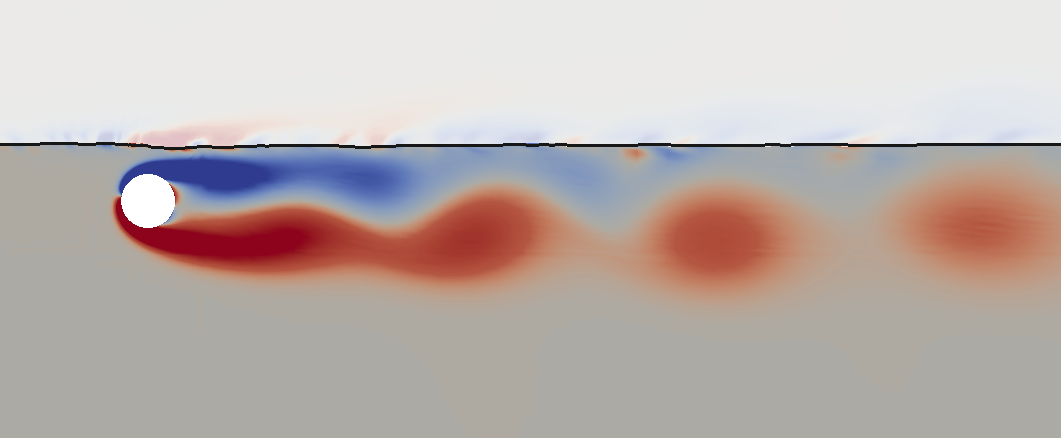
\includegraphics[width=.9\columnwidth]{images_10thspheric/Fr_0_3_Re_180_h_0_55_vorticity.png}
    } \\
\subfloat[$Fr=0.6$]{
	  \label{fg:vort_b}
	  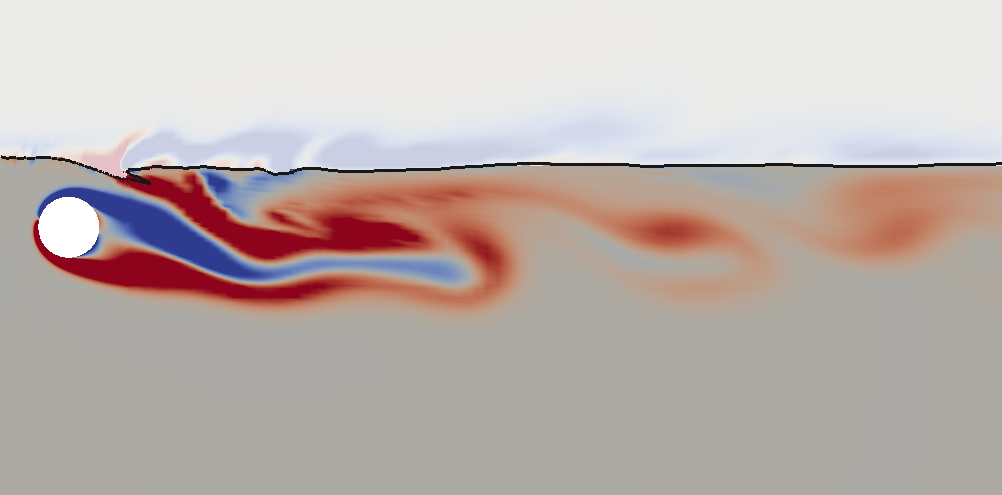
\includegraphics[width=.9\columnwidth]{images_10thspheric/Fr_0_6_Re_180_h_0_55_vorticity.png}
    } \\
\subfloat[$Fr=0.8$]{
	  \label{fg:vort_c}
	  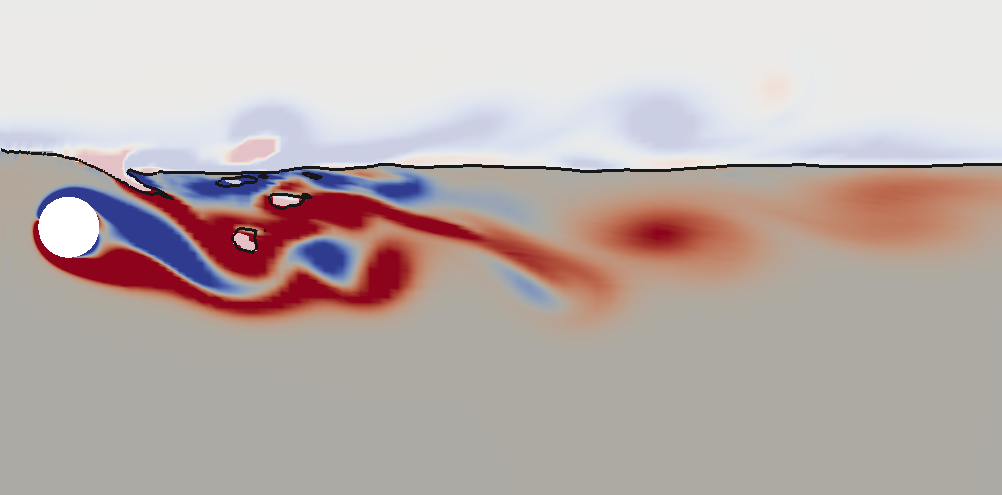
\includegraphics[width=.9\columnwidth]{images_10thspheric/Fr_0_8_Re_180_h_0_55_vorticity.png}
    } \\
\subfloat[$Fr=1.2$]{
	  \label{fg:vort_d}
	  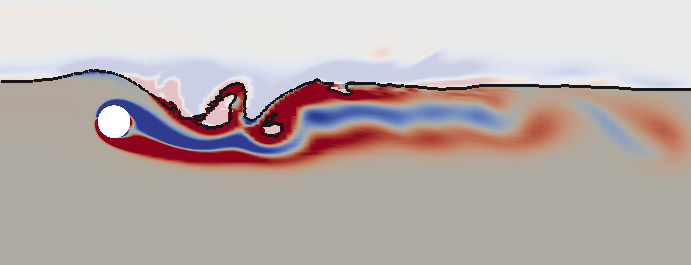
\includegraphics[width=.9\columnwidth]{images_10thspheric/Fr_1_2_Re_180_h_0_55_vorticity.png}
    } \\
\subfloat[$Fr=1.6$]{
	  \label{fg:vort_e}
	  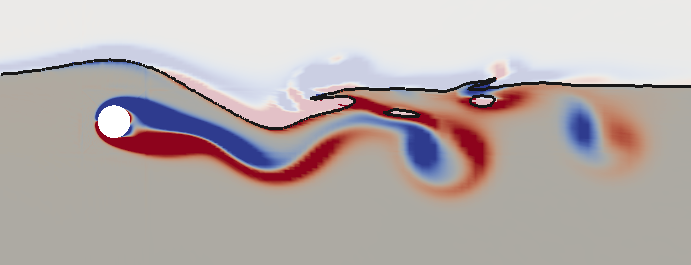
\includegraphics[width=.9\columnwidth]{images_10thspheric/Fr_1_6_Re_180_h_0_55_vorticity.png}
    } \\
\subfloat[$Fr=2.0$]{
	  \label{fg:vort_f}
	  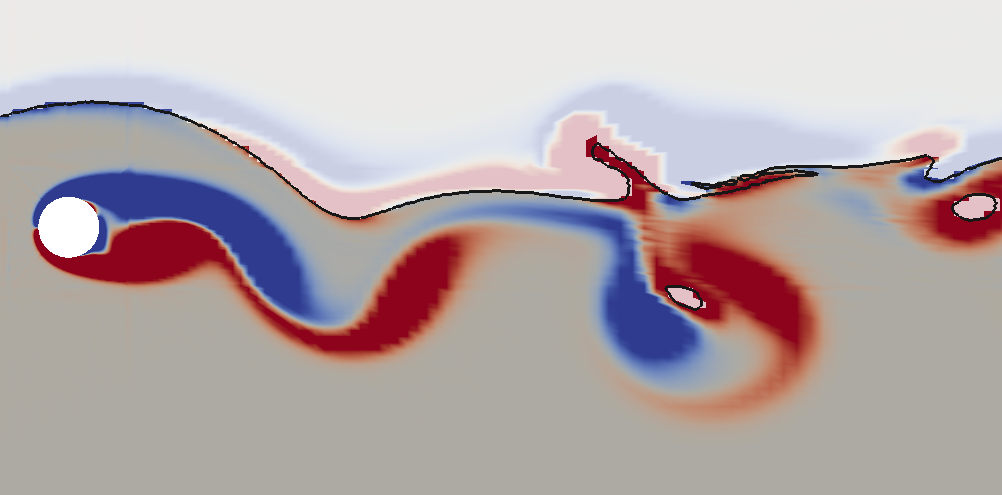
\includegraphics[width=.9\columnwidth]{images_10thspheric/Fr_2_0_Re_180_h_0_55_vorticity.png}
    } \\
% \subfloat[$Fr=3.5$]{
% 	  \label{fg:vort_g}
% 	  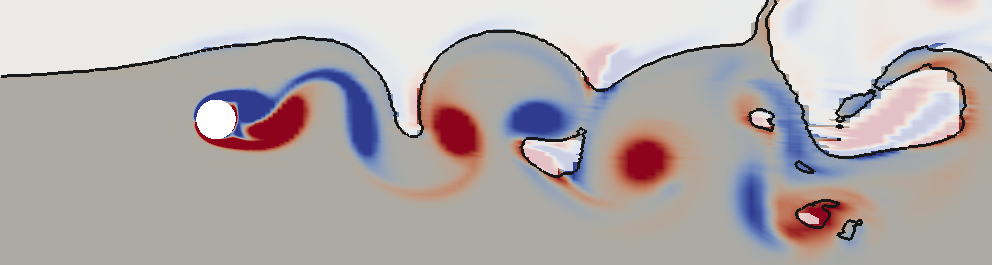
\includegraphics[width=.9\columnwidth]{images_10thspheric/Fr_3_5_Re_180_h_0_55_vorticity.png}
%     } \\
  \end{center}
  \caption{Influence of Froude number on dimensionless vorticity $\hat\omega = curl(\vv) \sqrt{d/g}$ (scales from -3 (blue) to 3 (red)) with $h/d = 0.55$ and $Re=180$. Captures at $t^*=80$.
}
\label{fg:vort_Re180}
\end{figure}

Flow conditions are inspirated in the work of Bouscasse \cite{Bouscasse14} which investigates the flow behavior employing a range of Froude numbers ($Fr=0.3$, $0.6$, $0.8$, $1.2$, $1.6$ and $2.0$) for a fixed submergence ratio ($h/d=0.55$) and a fixed Reynolds number of $Re=\frac{\rho_l U d}{\mu_l}=180$.

As it was explained in the introduction, one of the advantages of using SPH as numerical method allowing is to treat larger fragmentation of the free surface, when compared to FLUENT-VOF technique used by Reichl and colleagues. The PFEM-2 method employed in the current work, since its particle nature, is also able to treat large deformations and breakups, but, due to the use of the temporal integrator named XIV-S \cite{Idelsohn12}, it can manage larger time steps resulting in shorter computing times \cite{Gimenez2015186}. PFEM-2 simulations were carried out employing the implementation presented in \cite{Gimenez14}. The maximum $CFL=\Delta t U/\Delta x$ allowed in each simulation was $CFL_{max}<8$, in contrast with the small time-steps typically needed by SPH. This feature entails a diminishing in the total computing time to solve the same problem, showing the goodness given by PFEM-2 to solve convective-dominant problems.

\subsection{Simulation Results}

Figure \ref{fg:vort_Re180} shows the influence of the Froude number in the flow characteristics, represented by the dimensionless vorticity. Due to the PFEM-2 is a two-phase solver, in the plots the air regions are presented with some transparency in order to remark the water regions. When the lowest Froude number is imposed $Fr=0.3$, the free-surface deforms very little behaving as a no-slip wall where the vorticity presents a distribution similar to the cases where only one-phase is used \cite{PRICE2002175}. As the Froude number increases $Fr=0.6$, the velocity and vorticity fields change substantially. Although the free-surface just deforms in the proximities of the cylinder, the vortex shedding process has been substantially reduced. Another important observation is that, a recirculation area appears just behind the cylinder and close to the free-surface, the positive vorticity generated at the free surface by the spilling breaker builds up a large positive meta-vortex behind the cylinder which is then advected downstream. Reaching intermediate-high Froude numbers (1.2) structures developed are not periodic, while as the vortex production remains blocked due to the continuous breakups occurring at free-surface. Although the non-stationary behavior of the flow at free-surface, this phenomena allows to obtain constant forces acting over the cylinder. Analysis and discussions presented in this paragraph are in agreement with the work of Bouscasse et. al \cite{Bouscasse14}.

When the analysis for $Fr=1.6$ is done, some differences between the flow characteristics of Bouscasse et. al \cite{Bouscasse14} and the present work are found. Bouscasse shows that at this Froude number the vortex shedding remains blocked while the current results find that it is almost recovered. In order to present a regime where a structure similar to a Von Karman street appears, cases with $Fr=2.0$ and $3.5$ were also run finding vortex shedding behind the cylinder and large distortions of the free-surface but without the characteristic chaos of the intermediate Froude numbers. For the case of $Fr=2.0$, Bouscasse also recovers the shedding production in his simulations, showing similar results with our simulation. In order to confirm if there is any dependence between the Froude number and the transition from a convective to an absolute instability in the cylinder flow, next section presents a stability analysis study using the Froude number as principal parameter.

A summary of computed force coefficients can be seen in Fig. \ref{fg:CdCl}. The drag and lift coefficients, calculated as $Cd=2 F_x/(\rho_l U^2 d)$ and $Cl=2 F_y/(\rho_l U^2 d)$ where $F_x$ and $F_y$ are the projection on the inflow and normal inflow directions respectively of the global $\mathbf{F}$ force over the cylinder due to pressure and viscous effects. At each case, the drag and lift coefficients represent the temporal average for the computed case, and the bars shows the periodic variability of the amplitude. The lift coefficient, calculated as where  is the projection on the inflow direction of the global $\mathbf{F}$ force over the cylinder due to pressure and viscous effects. We can observe that $Cd$ decreases when the Froude number is increased. The maximum value of the lift coefficient (in absolute value) is found between $Fr = 0.6 - 0.8$, and then a gentle monotonic reduction for the largest Froude number cases occurs. Only in the cases where the vortex shedding is not blocked, appreciable amplitude variation can be observed. Mean values and the majority of the amplitude variations present good agreement with the referenced work \cite{Bouscasse14}.

\begin{figure}[ht]
  \centering
  %%----primera subfigura----
  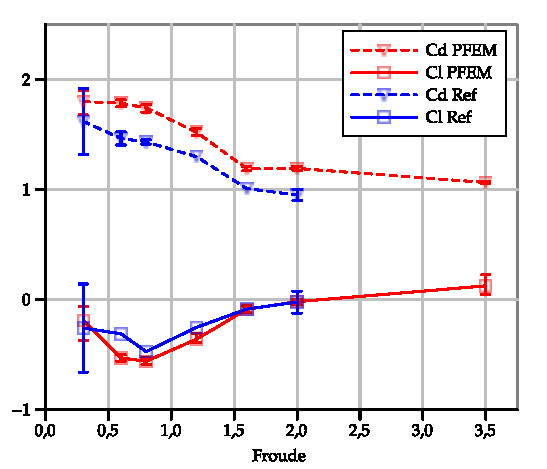
\includegraphics[width=0.95\columnwidth]{images_10thspheric/CdCl_Re180_hd_0_55.pdf}
  \caption{Drag and Lift coefficients calculated with PFEM-2 compared with the reference work of Bouscasse \cite{Bouscasse14}. $Re=180$.} %, $t^*=tU/d$. }
  \label{fg:CdCl}
\end{figure}

\subsection{DMD-Analysis Results}

\begin{figure}[ht]
  \centering
  %%----primera subfigura----
  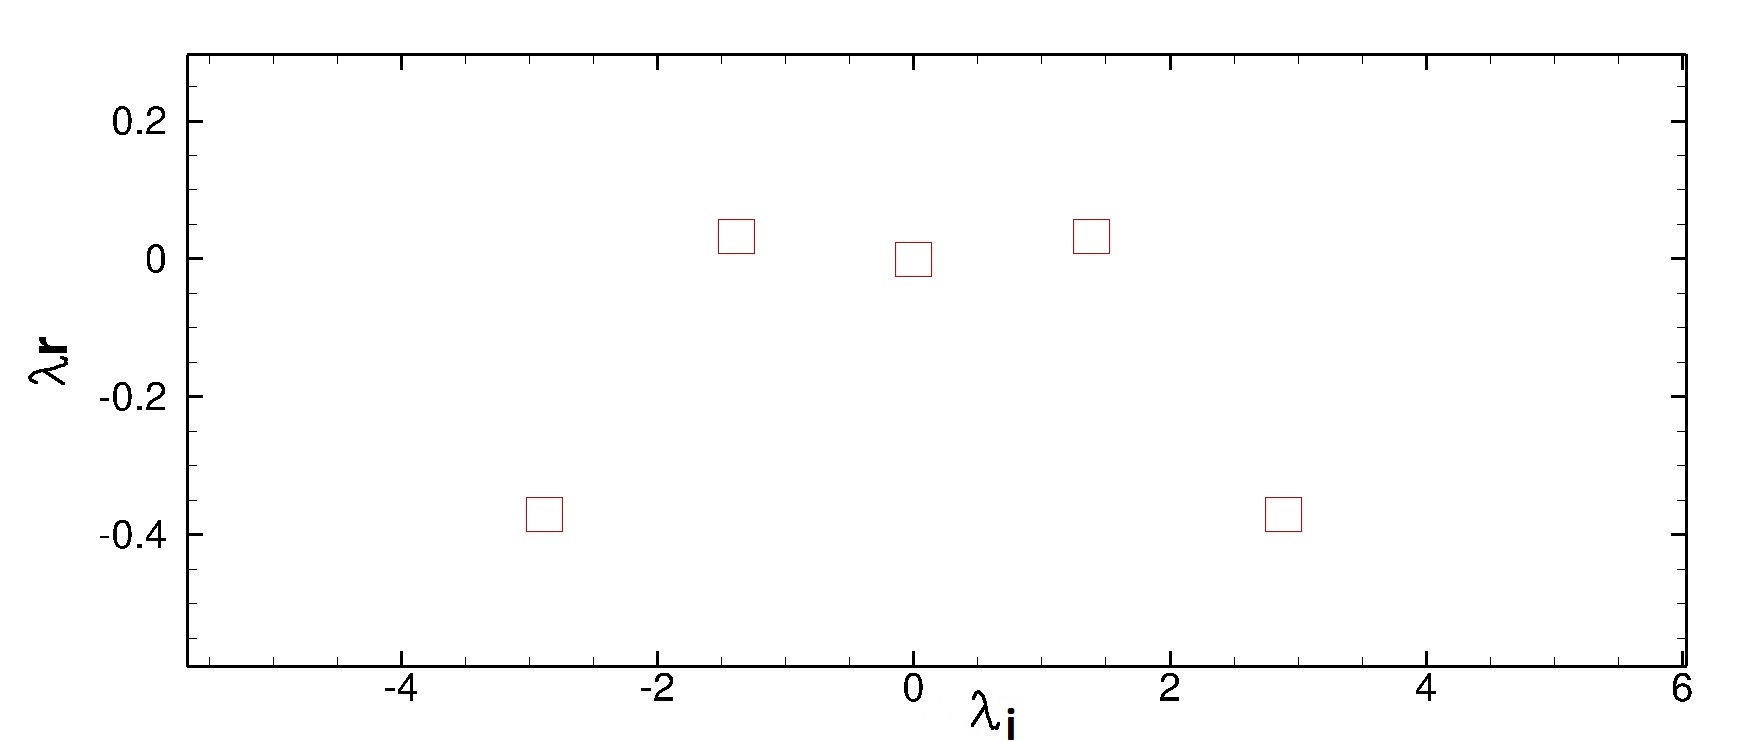
\includegraphics[width=0.95\columnwidth]{images_10thspheric/modos2.jpeg}
  \caption{Spectrum obtained after the DMD analysis when 7 snapshots spaced $\Delta t=0.48$ in the time interval $[11.99,15.51]$ equivalent to $\sim0.7T$ were used at $Fr=3.5$ and $Re=180$.}
  \label{fg:DMD_spectrum}
\end{figure}

\begin{figure}[ht]
  \centering
  %%----primera subfigura----
  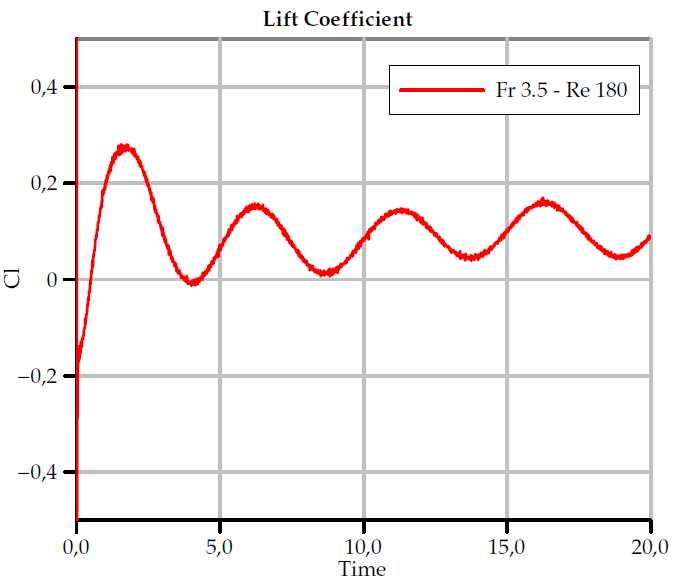
\includegraphics[width=0.95\columnwidth]{images_10thspheric/ClvstimeFr035.png}
  \caption{Evolution in time of the lift coefficient $C_l$ at $Fr=3.5$ and $Re=180$ when 20s are simulated.}
  \label{fg:Liftversustime}
\end{figure}

Different DMD analyses were done for the case $Re=180$ and $Fr=3.5$, in the first case 7 snapshots spaced $\Delta t=0.48$ in the time interval $[11.99,15.51]$ equivalent to $\sim0.7T$ were used, being $T\sim5s$ the dominant period of the flow. The most relevant part of the spectrum is shown in figure \ref{fg:DMD_spectrum}, where due to the fact that the the reduced matrix $\mathbf{\widetilde{S}}$ is real, all the eigenvalues are complex conjugate. It can be observed that a pair of eigenvalues have real positive part which means that a growing instability is present in the fluid. This growing stability is not conclusive and only comes from the fact that the set of snapshots do not complete a full period, capturing the slight increasing slope when the interval $[11.99,15.51]$ is observed in figure \ref{fg:Liftversustime}, which implies a positive real part. However the imaginary part associated with the most unstable eigenvalue is $1.27$ which corresponds to a period $2\pi/\lambda_i=4.94$, which fits very well 
with the one presented in the lift coefficient evolution $T\sim5s$, see figure \ref{fg:Liftversustime}. The perturbation components associated with this dominant eigenvalue $(\lambda_r,\lambda_i)=(0.05,1.5)$ are plot in figure \ref{fg:mode}, where the typical shape associated to a vortex shedding mode can be observed. To the authors knowledge this is the first time where a typical vortex shedding mode is observed in the presence of free surface. It can be observed how the mode is deformed due to the free surface shape when compared to the typical vortex shedding mode when no free surface has been introduced, see figure \ref{fg:mode Nofreesurface} from a typical biglobal computation at $Re=60$. A second DMD analysis was performed using 40 snapshots spaced $\Delta t=0.16$ in the time interval $[11.9,18.3]$ equivalent to $\sim 1.3T$, in this case the most dominant mode shifted its real part to the stable part of the spectrum, while the frequency is fixed to similar to the ones obtained in the first case. The 
decrease of the real part of the dominant mode can be explained due to the fact that the snapshots have been taken during a longer interval where the growing tendency is not so clearly observed. However the structure of the mode barely changes as can be appreciated when figures \ref{fg:DMDglobal2} and \ref{fg:DMDglobal3} are compared. Finally, a third analysis 20 snapshots spaced $\Delta t=0.5$ in the time interval $[19.98,30.48]$ equivalent to $\sim2T$ were used. If the total simulation time is extended from 20s to 50s, the growing tendency of the lift coefficient is clearly observed, see figure \ref{fg:Liftlonger}. The result from the DMD analysis captures this growing tendency and shifts the dominant mode back to the unstable part of the plane $\lambda_r<0$, see figure \ref{fg:DMDglobal} keeping the frequency of the mode at similar values as the previous analyses. As before, the structure of the dominant mode reamins unchanged, see figure \ref{fg:DMDglobal4}. The complexity of the flow can be appreciated 
when a secondary mode is plot, see figure \ref{fg:DMDglobal5}, where the higher temporal frequency implies a more complex structure in the mode.



\begin{figure}[ht]
  \centering
  %%----primera subfigura----
  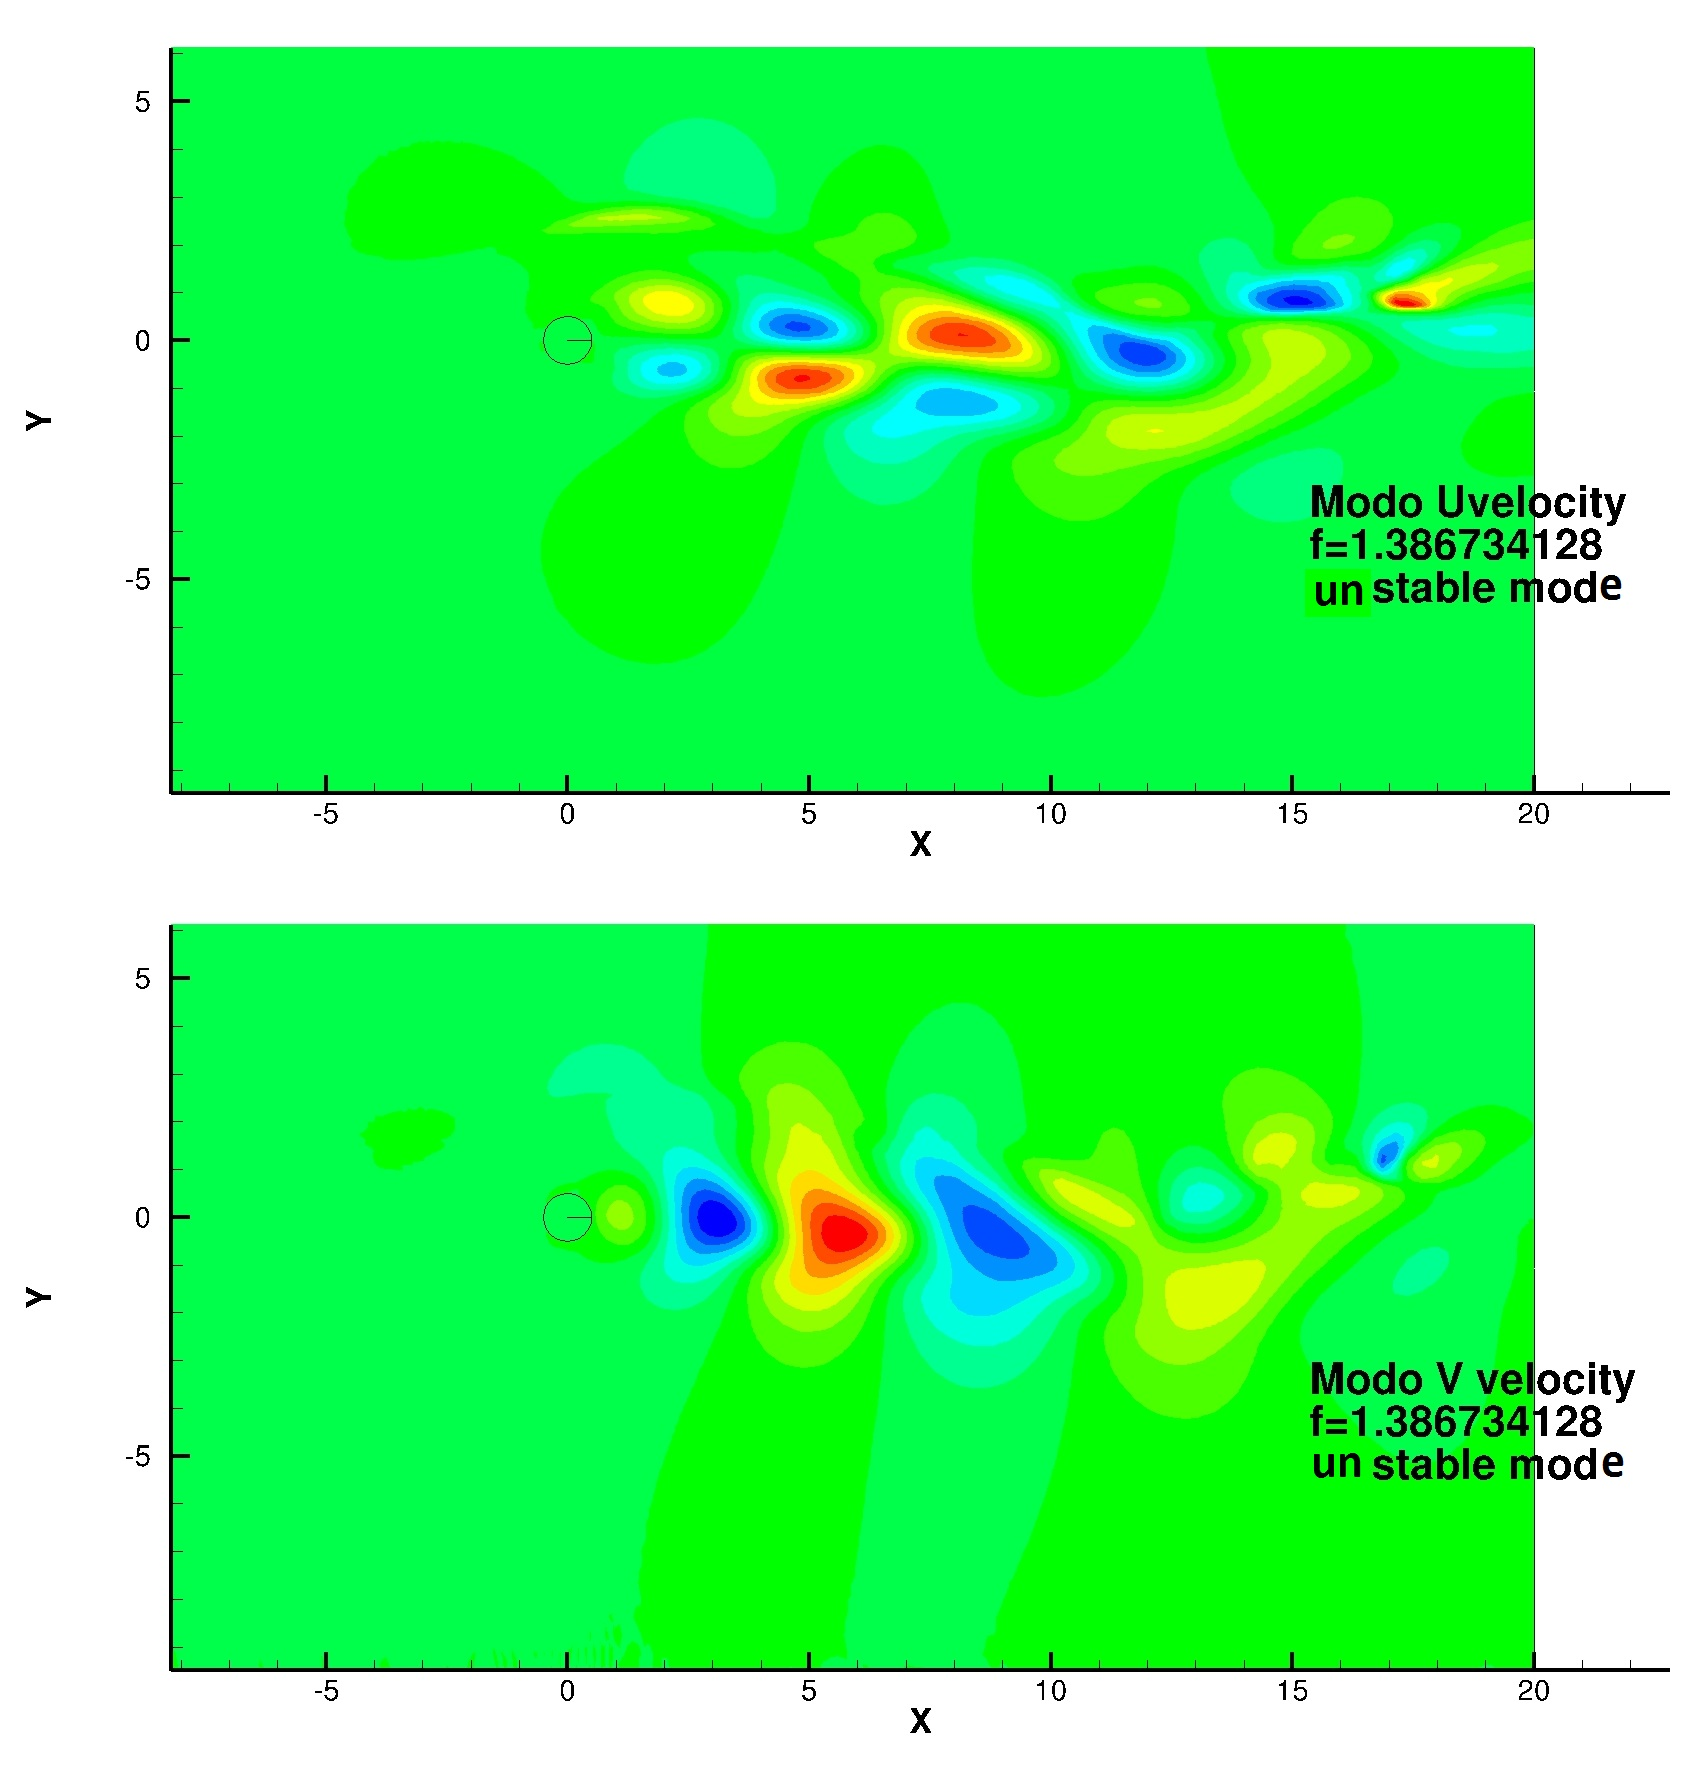
\includegraphics[width=1\columnwidth]{images_10thspheric/modos3.jpeg}
  \caption{Perturbation velocity components of the most unstable mode obtained after the first DMD analysis when 7 snapshots spaced $\Delta t=0.48$ in the time interval $[11.99,15.51]$ equivalent to $\sim0.7T$ at $Fr=3.5$ and $Re=180$. Top: horizontal velocity, bottom: vertical velocity component.}
  \label{fg:mode}
\end{figure}

\begin{figure}[ht]
  \centering
  %%----primera subfigura----
  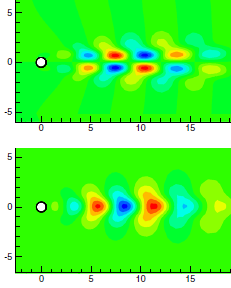
\includegraphics[width=0.95\columnwidth]{images_10thspheric/Typical_cilinder_mode.png}
  \caption{Perturbation velocity components of the most unstable mode obtained by biglobal analysis when the $Re=60$ and no free surface has been considered. Top: horizontal velocity, bottom: vertical velocity component.}
  \label{fg:mode Nofreesurface}
\end{figure}

\begin{figure}[ht]
  \centering
  %%----primera subfigura----
  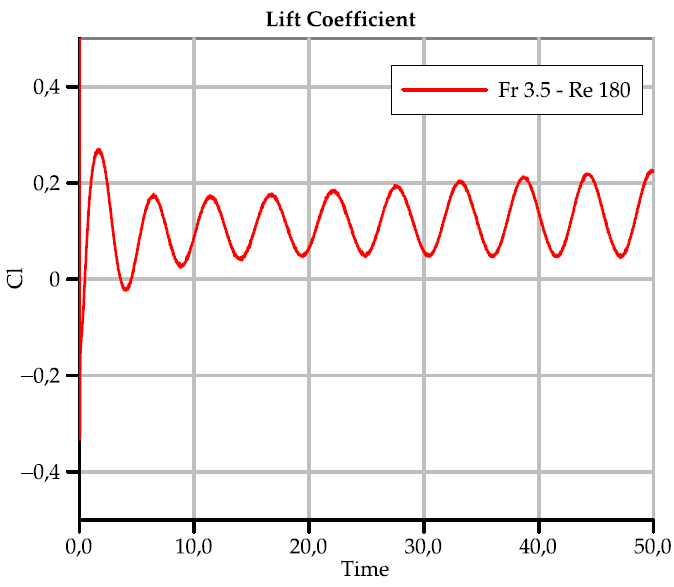
\includegraphics[width=0.95\columnwidth]{images_10thspheric/LongerCl.png}
  \caption{Evolution in time of the lift coefficient $C_l$ at $Fr=3.5$ $Re=180$ when 50s are simulated.}
  \label{fg:Liftlonger}
\end{figure}

\begin{figure}[ht]
  \centering
  %%----primera subfigura----
  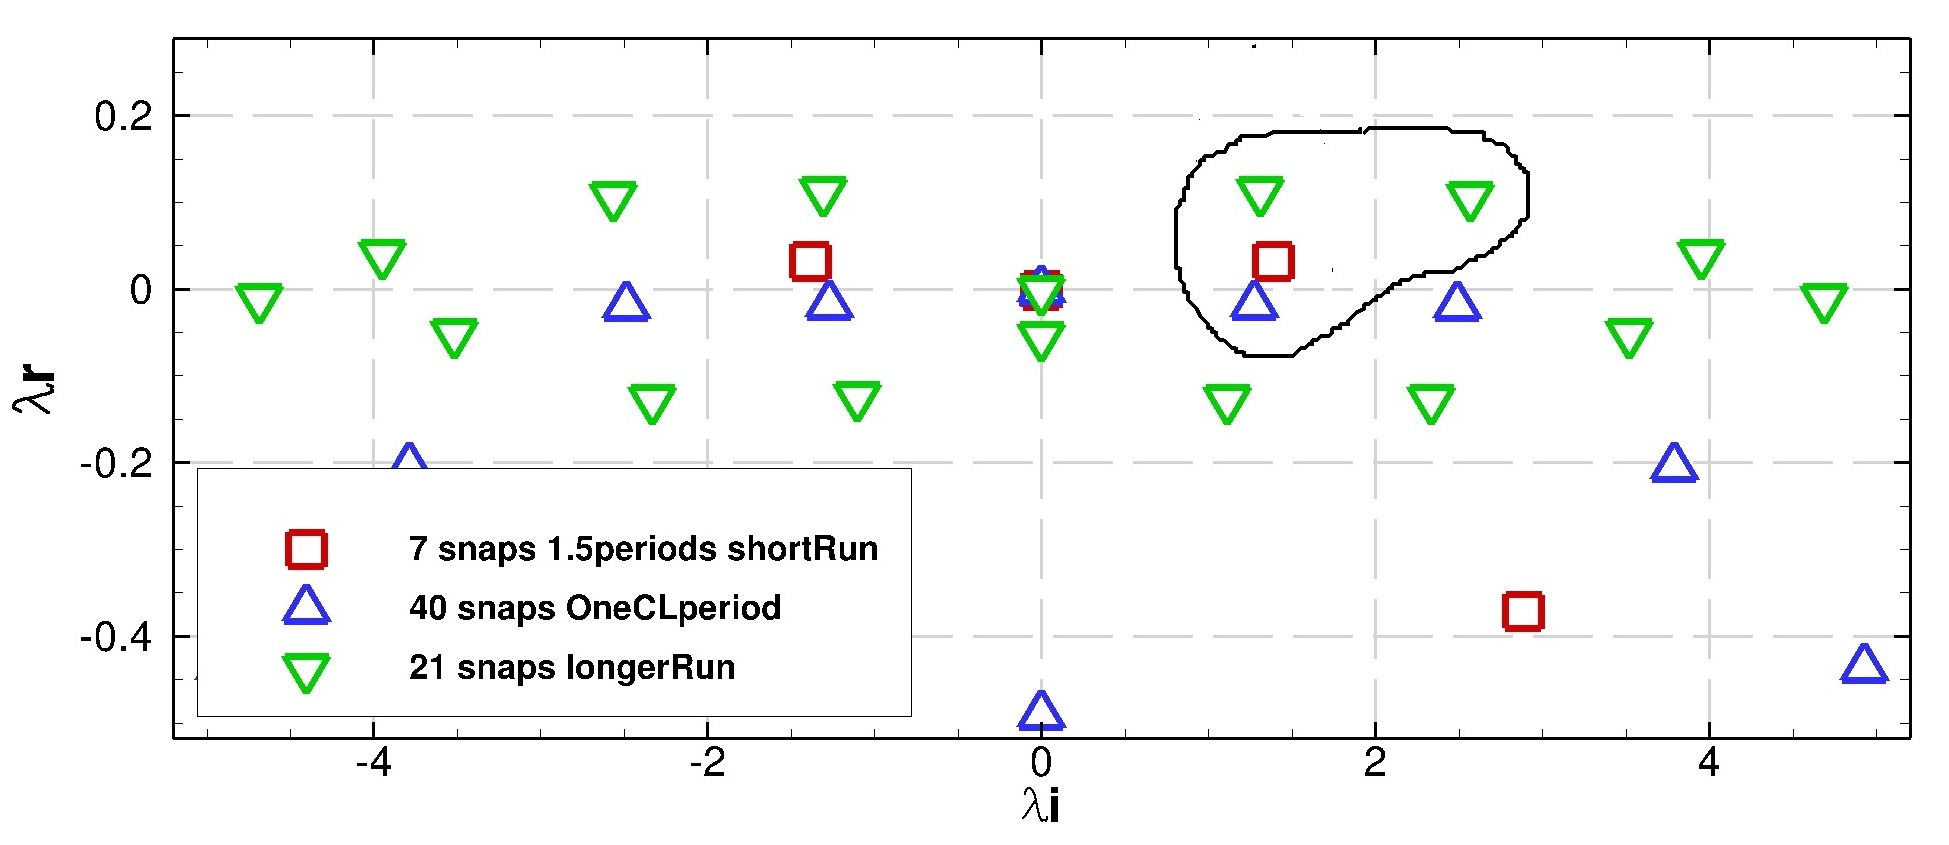
\includegraphics[width=0.95\columnwidth]{images_10thspheric/7vs40vslongersnaps.jpg}
  \caption{Comparative spectra obtained after the three DMD analysis at $Fr=3.5$ and $Re=180$}
  \label{fg:DMDglobal}
\end{figure}

\begin{figure}[ht]
  \centering
  %%----primera subfigura----
  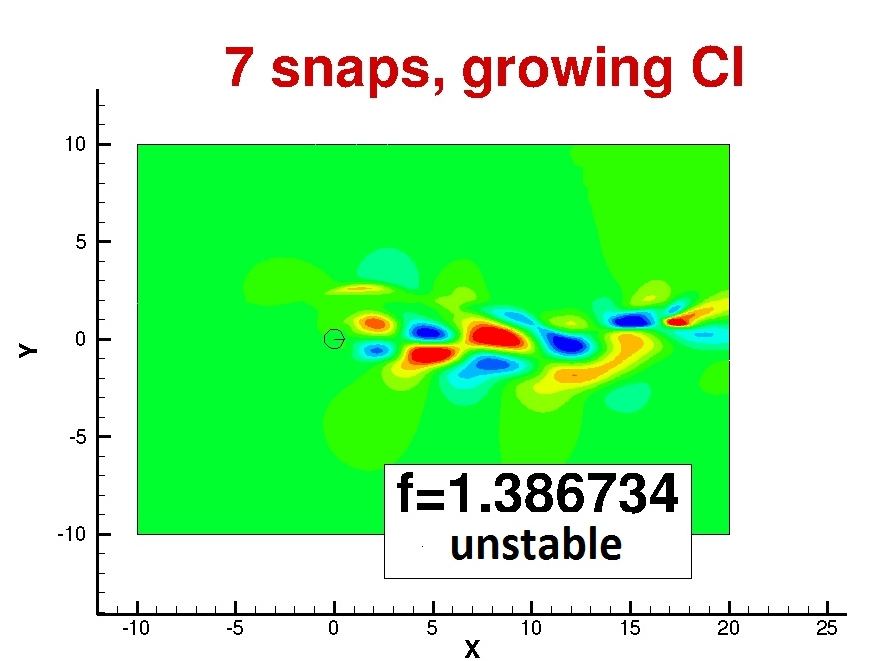
\includegraphics[width=0.95\columnwidth]{images_10thspheric/modo1u.png}
  \caption{Horizontal velocity component of the unstable mode represented by a red square inside the rounded area in figure \ref{fg:DMDglobal}.}
  \label{fg:DMDglobal2}
\end{figure}
\begin{figure}[ht]
  \centering
  %%----primera subfigura----
  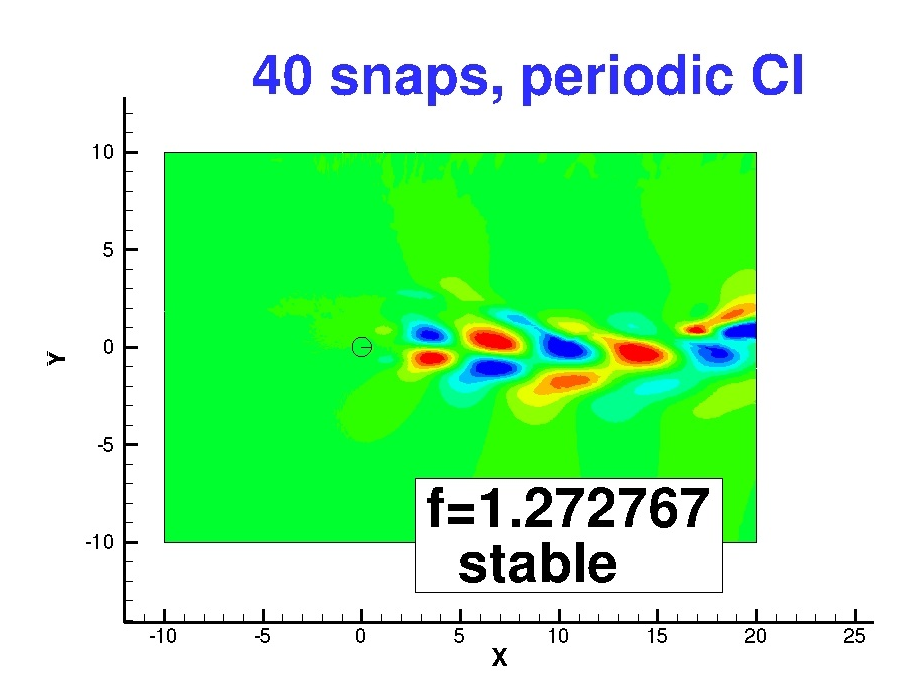
\includegraphics[width=0.95\columnwidth]{images_10thspheric/modo2u.png}
  \caption{Horizontal velocity component of the stable mode represented by a blue triangle inside the rounded area in figure \ref{fg:DMDglobal}.}
  \label{fg:DMDglobal3}
\end{figure}

\begin{figure}[ht]
  \centering
  %%----primera subfigura----
  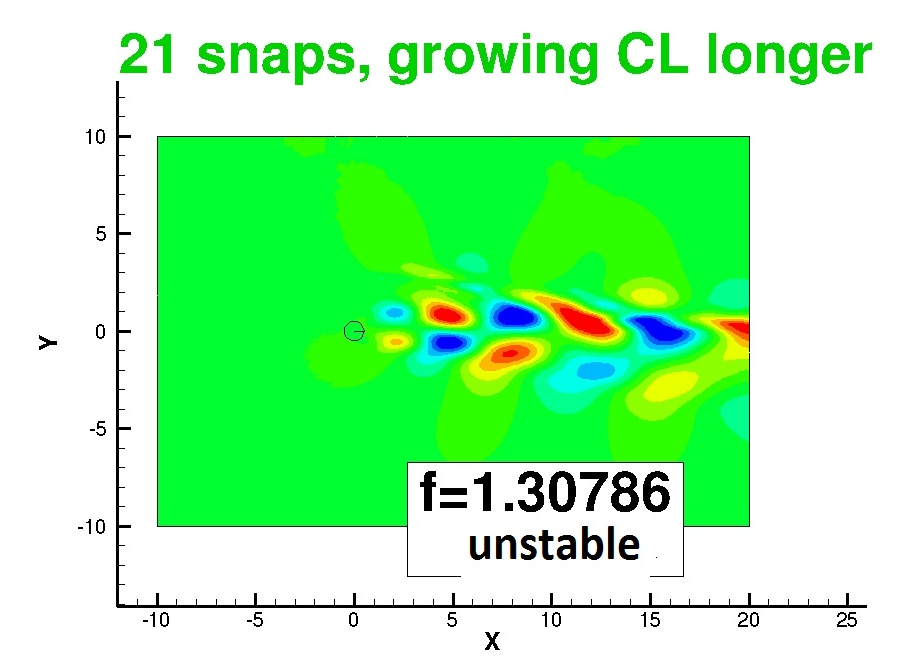
\includegraphics[width=0.95\columnwidth]{images_10thspheric/modo3u.png}
  \caption{Horizontal velocity component of the most unstable mode represented by a green triangle inside the rounded area in figure \ref{fg:DMDglobal}.}
  \label{fg:DMDglobal4}
\end{figure}
\begin{figure}[ht]
  \centering
  %%----primera subfigura----
  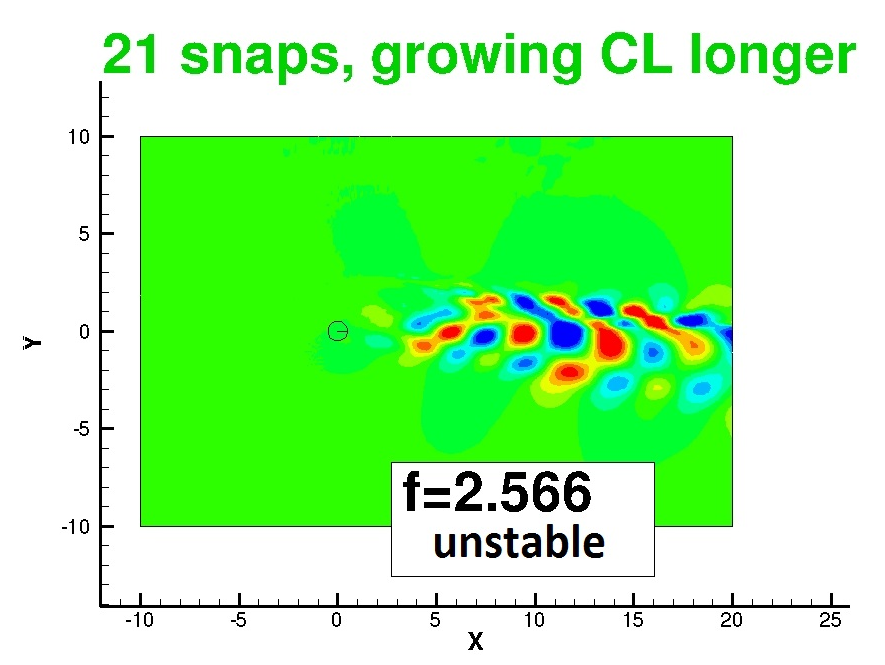
\includegraphics[width=0.95\columnwidth]{images_10thspheric/modo4u.png}
  \caption{Horizontal velocity component of the secondary unstable mode represented by a green triangle inside the rounded area in figure \ref{fg:DMDglobal}.}
  \label{fg:DMDglobal5}
\end{figure} 


\section{Conclusion}
The last generation of the Particle Finite Element Method (PFEM-2) is a contemporary strategy which uses a spatial discretization based on a background mesh and a cloud of particles. The dynamics equations are solved in a Lagrangian frame, where the implicit non-linearities of the equation are solved using the X-IVAS strategy. That explicit temporal integration for convective terms allows for the use of large time-steps, thus providing a very efficient way when computing times are concerned.
In the current work, a formulation to solve a particular free-surface flows such as a submerged cylinder has been tested. The algorithm has shown good accuracy when solving this complex problem with large free surface deformations while keeping the advantage of using large time-steps. A large variety of Froude numbers have been analyzed and good agreement in terms of drag and lift mean values and amplitudes have been obtained when the results have been compared to other specific numerical methods for free surface flows such as SPH. In each of them, PFEM-2 has proven to be accurately competitive and computationally efficient.
In addition, the recently develop Dynamic Mode Decomposition technique, has shown to be an efficient, robust and cost effective mean to extract dynamical information from snapshots produced by PFEM-2 computations. This technique expands the potential of this type of analysis based on snapshot analysis to existing
Computational Fluid Dynamics (CFD) codes, without need of modifications. The DMD analysis confirms the presence of flow instability when the cylinder is simulated at $Fr=3.5$ and $Re=180$, in the line the results presented in previous publications, see \cite{Dimas89}.

% use section* for acknowledgement
\section*{Acknowledgment}
Authors thank the program ERASMUS MUNDUS action 2 ARCOIRIS project for financial support through a six-month doctoral scholarship. The research leading to these results has received funding from the Spanish Ministry for Science and Innovation under grant TRA2013-41096-P
"Optimization of liquid gas transport for LNG vessels by fluid structure interaction studies"

\bibliographystyle{plain}
\bibliography{mybib}


\end{document}


